% \documentclass[aspectratio=169]{beamer}
% \usepackage{beamerstyle}

% \begin{document}

\begin{frame}
	\vspace{2cm}
	\begin{center}
		{\Huge\textbf{\textcolor{copenhagenred}{Parallel Tempering MCMC}}}
		\vspace{1cm}

		\rule{4cm}{3pt}
		\vspace{2cm}
	\end{center}
\end{frame}

\begin{frame}{The Problem and Solution}

	\begin{columns}
		\column{0.48\textwidth}
		\textbf{The Problem:}
		\begin{itemize}
			\item Standard MCMC gets stuck in local modes
			\item Can't explore separated peaks
			\item Dilemma: small steps (stuck) vs. large steps (rejected)
		\end{itemize}

		\textbf{The Solution: Temperature Ladder}
		\begin{itemize}
			\item Run $N$ chains targeting $\pi^{\gamma_n}$
			\item $0 < \gamma_1 < \cdots < \gamma_N = 1$
			\item \textcolor{red}{Hot ($\gamma \approx 0$)}: Explores freely
			\item \textcolor{blue}{Cold ($\gamma = 1$)}: Exploits peaks
		\end{itemize}

		\column{0.48\textwidth}
		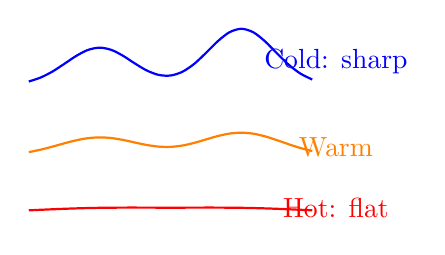
\begin{tikzpicture}[scale=0.6]
			% Hot chain
			\draw[red,thick] plot[smooth,domain=-3:3] (\x,{0.3 + 0.1*exp(-(\x+1.5)^2/4) + 0.1*exp(-(\x-1.5)^2/4)});
			\node[red] at (3.5,0.4) {Hot: flat};

			% Medium chain  
			\draw[orange,thick] plot[smooth,domain=-3:3] (\x,{1.5 + 0.4*exp(-(\x+1.5)^2/1.5) + 0.5*exp(-(\x-1.5)^2/1.5)});
			\node[orange] at (3.5,1.7) {Warm};

			% Cold chain
			\draw[blue,thick] plot[smooth,domain=-3:3] (\x,{3 + 0.8*exp(-(\x+1.5)^2) + 1.2*exp(-(\x-1.5)^2)});
			\node[blue] at (3.5,3.5) {Cold: sharp};

			% % Show modes
			% \node at (-1.5,2.5) {A};
			% \node at (1.5,3.2) {B};
		\end{tikzpicture}

		% \vspace{0.2cm}
		% \begin{center}
		% 	\begin{tikzpicture}[scale=0.5, node distance=0.8cm]
		% 		\node[circle,draw,red] (hot) {Hot};
		% 		\node[circle,draw,orange,right of=hot] (warm) {Warm};
		% 		\node[circle,draw,blue,right of=warm] (cold) {Cold};
		% 		\draw[<->,thick] (hot) -- (warm);
		% 		\draw[<->,thick] (warm) -- (cold);
		% 	\end{tikzpicture}
		% \end{center}
	\end{columns}

			\vspace{0.2cm}
	\textbf{Key Insight}
		Different temperatures see the same distribution differently - hot chains explore, cold chains exploit

\end{frame}

% \begin{frame}{The Challenge: Multimodal Distributions}
% 	\begin{columns}
% 		\column{0.5\textwidth}
% 		\textbf{Standard MCMC Problems:}
% 		\begin{itemize}
% 			\item Gets trapped in local modes
% 			\item Exponentially slow mixing times
% 			\item Poor exploration of state space
% 			\item Fails to discover all modes
% 		\end{itemize}



% 		\column{0.5\textwidth}
% 		\begin{tikzpicture}[scale=0.8]
% 			\begin{axis}[
% 					xlabel={$x$},
% 					ylabel={$\pi(x)$},
% 					ymin=0, ymax=1.2,
% 					xmin=-4, xmax=4,
% 					height=6cm,
% 					width=8cm,
% 					grid=major,
% 					legend pos=north east
% 				]
% 				% Multimodal distribution
% 				\addplot[copenhagenred, thick, samples=200, domain=-4:4]
% 				{0.3*exp(-2*(x+2)^2) + 0.7*exp(-2*(x-1.5)^2)};
% 				\addlegendentry{Target $\pi(x)$}

% 				% MCMC trace stuck in one mode
% 				\addplot[darkgray, thick, dashed, samples=50, domain=0.5:2.5]
% 				{0.7*exp(-2*(x-1.5)^2)};
% 				\addlegendentry{MCMC exploration}
% 			\end{axis}
% 		\end{tikzpicture}

% 	\end{columns}
% \end{frame}


\begin{frame}{The Temperature Mechanism}
	\begin{block}{Key Idea: Tempered Distributions}
		Define a family of distributions indexed by inverse temperature $0 < \gamma_1 < \gamma_2 < \ldots < \gamma_N = 1$:
		$$\pi_{\gamma_n}(x) \propto \pi(x)^{\gamma_n}$$
		where $n=1, \ldots, N$ and $\pi(x)$ is our target distribution.
	\end{block}

	\begin{columns}
		\column{0.5\textwidth}
		\textbf{Properties:}
		\begin{itemize}
			\item $\gamma_N = 1$: Original target distribution
			\item $\gamma_N \approx 0$: Uniform, explores broadly
		\end{itemize}

		\column{0.5\textwidth}
		\begin{tikzpicture}[scale=0.7]
			\begin{axis}[
					xlabel={$x$},
					ylabel={$\pi_T(x)$},
					ymin=0, ymax=1,
					xmin=-4, xmax=4,
					height=5cm,
					width=7cm,
					legend pos=north east,
					cycle list name=color list
				]
				% Different temperatures
				\addplot[copenhagenred, thick, samples=100, domain=-4:4]
				{0.3*exp(-2*(x+2)^2) + 0.7*exp(-2*(x-1.5)^2)};
				\addlegendentry{$T=1$}

				\addplot[copenhagenred!70, thick, dashed, samples=100, domain=-4:4]
				{(0.3*exp(-2*(x+2)^2) + 0.7*exp(-2*(x-1.5)^2))^(1/2)};
				\addlegendentry{$T=2$}

				\addplot[copenhagenred!40, thick, dotted, samples=100, domain=-4:4]
				{(0.3*exp(-2*(x+2)^2) + 0.7*exp(-2*(x-1.5)^2))^(1/4)};
				\addlegendentry{$T=4$}
			\end{axis}
		\end{tikzpicture}
	\end{columns}
\end{frame}

\begin{frame}{Parallel Chains Architecture}
	\begin{center}
		\begin{tikzpicture}[scale=0.9]
			% Draw chains
			\foreach \i in {1,...,4} {
					\draw[thick, darkgray] (0, \i*1.5) -- (10, \i*1.5);
					\node[left] at (0, \i*1.5) {Chain \i};
				}

			% Temperature labels
			\node[right, copenhagenred] at (10, 1.5) {$T_1 = 1.0$ (target)};
			\node[right, copenhagenred] at (10, 3) {$T_2 = 1.5$};
			\node[right, copenhagenred] at (10, 4.5) {$T_3 = 2.25$};
			\node[right, copenhagenred] at (10, 6) {$T_4 = 3.38$};

			% States on chains
			\foreach \x in {1,2,...,9} {
					\foreach \y in {1,...,4} {
							\fill[copenhagenred!70] (\x, \y*1.5) circle (0.1);
						}
				}

			% Swap moves
			\draw[<->, thick, copenhagenred] (3.5, 1.8) -- (3.5, 2.7);
			\node[right, font=\small] at (3.6, 2.25) {swap};

			\draw[<->, thick, copenhagenred] (6.5, 3.3) -- (6.5, 4.2);
			\node[right, font=\small] at (6.6, 3.75) {swap};

			% Within-chain moves
			\draw[->, thick, darkgray] (1.1, 1.5) -- (1.9, 1.5);
			\draw[->, thick, darkgray] (4.1, 3) -- (4.9, 3);
		\end{tikzpicture}
	\end{center}

	% \vspace{0.1cm}
	\begin{block}{Two Types of Moves}
		\begin{enumerate}
			\item \textbf{Within-chain updates}: Standard MCMC at each temperature
			\item \textbf{Between-chain swaps}: Exchange states between adjacent temperatures
		\end{enumerate}
	\end{block}
\end{frame}

\begin{frame}{Parallel Tempering Algorithm Prerquisites}
	\begin{itemize}
		\item \textbf{Target Distribution}: $\pi(x)$
		\item \textbf{Proposal Distribution}: For each tempered chain $q(x' | x)$ - could potentially depend on temperature
		\item \textbf{Initialization}: $x_n^{(0)}$ for $n = 1, \ldots, N$
		\item \textbf{Standard MCMC Step}: Any MCMC kernel (e.g., RWM, MALA)
		\item \textbf{Number of Chains}: $N$
		\item \textbf{Number of Samples per Chain}: $T$
		% \item \textbf{Swapping Interval}: $s$
		\item \textbf{Temperature Schedule}: $\{\gamma_n\}_{n=1}^N$ with $\gamma_N = 1$
	\end{itemize}
\end{frame}

\begin{frame}{Parallel Tempering Algorithm}
	\begin{algorithm}[H]
		\caption{Parallel Tempering MCMC}
		\begin{algorithmic}[1]
			\FOR{$t = 1$ \TO $T$}
			\FORALL{$n \in \{1, \ldots, N\}$ \textbf{ in parallel}}
			\STATE Sample $x_n^{(t)}$ using a standard MCMC step targeting $\pi^{\gamma_n}$
			\ENDFOR
			\STATE $k \sim \text{Uniform}\{1, \ldots, N-1\}$
			\STATE $\alpha_{\text{swap}} = \min\left\{1, \left(\frac{\pi(x_{k+1}^{(t)})}{\pi(x_k^{(t)})}\right)^{\gamma_k - \gamma_{k+1}}\right\}$
			\STATE Swap $(x_k^{(t)}, x_{k+1}^{(t)})$ with probability $\alpha_{\text{swap}}$
			\ENDFOR
			\RETURN $\{x_N^{(t)}\}_{t=1}^T$
		\end{algorithmic}
	\end{algorithm}
\end{frame}

\begin{frame}{Swap Acceptance Ratio Derivation}
	\textbf{Propose swap:} Exchange states $x_{k_1} \leftrightarrow x_{k_2}$ between chains $k_1$ and $k_2$

	\begin{align*}
		\alpha_{\text{swap}} = \frac{\text{Prob of proposed state}}{\text{Prob of current state}} & = \min\left\{1, \frac{\pi^{\gamma_{k_1}}(x_{k_2}) \cdot \pi^{\gamma_{k_2}}(x_{k_1})}{\pi^{\gamma_{k_1}}(x_{k_1}) \cdot \pi^{\gamma_{k_2}}(x_{k_2})}\right\}           \\
		                     & = \min\left\{1, \frac{[\pi(x_{k_2})]^{\gamma_{k_1}}}{[\pi(x_{k_2})]^{\gamma_{k_2}}} \cdot \frac{[\pi(x_{k_1})]^{\gamma_{k_2}}}{[\pi(x_{k_1})]^{\gamma_{k_1}}}\right\} \\
		                     & = \min\left\{1, [\pi(x_{k_2})]^{\gamma_{k_1} - \gamma_{k_2}} \cdot [\pi(x_{k_1})]^{\gamma_{k_2} - \gamma_{k_1}}\right\}                                               \\
		                     & = \min\left\{1, \frac{[\pi(x_{k_2})]^{\gamma_{k_1} - \gamma_{k_2}}}{[\pi(x_{k_1})]^{\gamma_{k_1} - \gamma_{k_2}}}\right\}
		= \min\left\{1, \left(\frac{\pi(x_{k_2})}{\pi(x_{k_1})}\right) ^{\gamma_{k_1} - \gamma_{k_2}}    \right\}
	\end{align*}
\end{frame}

\begin{frame}{Parallel Tempering: Swap Move Acceptance}
	\begin{block}{Metropolis-Hastings Derivation}
		\textbf{Joint target:} $\pi^{\gamma_1} \otimes \pi^{\gamma_2} \otimes \cdots \otimes \pi^{\gamma_N}$ where $\gamma_i$ (inverse temperature)

		\textbf{MH acceptance ratio:}
		$$\alpha = \frac{\text{Probability of proposed state}}{\text{Probability of current state}} = \frac{\pi^{\gamma_{k_1}}(x_{k_2})\pi^{\gamma_{k_2}}(x_{k_1})}{\pi^{\gamma_{k_1}}(x_{k_1})\pi^{\gamma_{k_2}}(x_{k_2})}$$

		\textbf{Accept with probability:} $\min(1, \alpha)$

		Swapping state of two chains doesn’t change the joint target distribution.
		This ensures detailed balance w.r.t. the joint distribution!
	\end{block}

	% \begin{columns}[t]
	% 	\begin{column}{0.48\textwidth}
	% 		\begin{block}{Intuition}
	% 			\begin{itemize}
	% 				\item \textcolor{red}{Hot chains}: Flat distribution, explore broadly
	% 				\item \textcolor{blue}{Cold chains}: Peaked distribution, exploit locally
	% 				\item Swaps likely when cold chain gets higher-probability state
	% 			\end{itemize}
	% 		\end{block}
	% 	\end{column}

	% 	\begin{column}{0.48\textwidth}
	% 		\begin{block}{Why It Works}
	% 			\begin{itemize}
	% 				\item Hot chains traverse energy barriers
	% 				\item Cold chain receives distant modes via swaps
	% 				\item Enables global moves impossible with standard MCMC
	% 			\end{itemize}
	% 		\end{block}
	% 	\end{column}
	% \end{columns}

\end{frame}


\begin{frame}{Parallel Tempering MCMC: Normalization Requirements}

	% \begin{block}{Key Question}
	% Do we need normalized distributions for parallel tempering MCMC?
	% \end{block}

	% \vspace{0.3cm}

	\begin{columns}[T]
		\begin{column}{0.48\textwidth}
			\begin{alertblock}{Target Distribution}
				\textbf{NOT required to be normalized}
				% \begin{itemize}
				%     \item Can work with $\pi(\mathbf{x}) = \frac{\tilde{p}(\mathbf{x})}{Z}$
				%     \item Only need $\tilde{p}(\mathbf{x})$ (unnormalized)
				%     \item $Z$ can be intractable
				% \end{itemize}
			\end{alertblock}
		\end{column}

		\begin{column}{0.48\textwidth}
			\begin{alertblock}{Tempered Distributions}
				\textbf{Also NOT normalized}
				% \begin{itemize}
				%     \item $\pi_i(\mathbf{x}) \propto \pi(\mathbf{x})^{1/T_i}$
				%     \item Temperature ladder: $T_1 = 1 < T_2 < \ldots < T_K$
				%     \item Each $\pi_i$ inherits unnormalized form
				% \end{itemize}
			\end{alertblock}
		\end{column}
	\end{columns}

	\vspace{0.4cm}

	\begin{block}{Why It Works: Acceptance Ratios}
		\begin{columns}[T]
			\begin{column}{0.45\textwidth}
				\textbf{Within-chain moves:}
				$$\alpha = \min\left(1, \frac{\pi_i(\mathbf{x}')}{\pi_i(\mathbf{x})}\right)$$
				\centering
				\textcolor{blue}{Normalizing constants cancel!}
			\end{column}
			\begin{column}{0.45\textwidth}
				\textbf{Between-chain swaps:}
				$$\alpha = \min\left(1, \frac{\pi_i(\mathbf{x}_j)\pi_j(\mathbf{x}_i)}{\pi_i(\mathbf{x}_i)\pi_j(\mathbf{x}_j)}\right)$$
				\centering
				\textcolor{blue}{Constants cancel again!}
			\end{column}
		\end{columns}
	\end{block}
\end{frame}

\begin{frame}{Why Swapping Works}

	\begin{columns}
		\column{0.55\textwidth}
		\textbf{The Relay Race Mechanism:}
		\begin{enumerate}
			\item \textcolor{red}{Hot chain} randomly discovers new mode
			\item Swap propagates discovery downward
			\item \textcolor{blue}{Cold chain} thoroughly explores it
			\item Information flows both ways
		\end{enumerate}

		\vspace{0.3cm}
		\textbf{Swap Acceptance (adjacent chains):}
		$$\alpha = \min\left\{1, \left(\frac{\pi(x_{k+1})}{\pi(x_k)}\right)^{\gamma_k - \gamma_{k+1}}\right\}$$

		\begin{itemize}
			\item Favors moving high-prob states to cold
			\item Favors moving low-prob states to hot
			\item Adjacent swaps → high acceptance
		\end{itemize}

		\column{0.45\textwidth}
		\textbf{Example: Two Islands}
		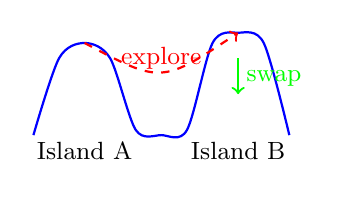
\begin{tikzpicture}[scale=0.65]
			% Distribution
			\draw[thick,blue] plot[smooth] coordinates {(-2.5,0) (-2,1.5) (-1.5,1.8) (-1,1.5) (-0.5,0.1) (0,0) (0.5,0.1) (1,1.8) (1.5,2) (2,1.8) (2.5,0)};
			\node at (-1.5,-0.3) {\small Island A};
			\node at (1.5,-0.3) {\small Island B};

			% Arrow showing hot chain path
			\draw[->,red,dashed,thick] (-1.5,1.8) .. controls (0,1) .. (1.5,2);
			\node[red] at (0,1.5) {\small explore};

			% Swap indication
			\draw[->,green,thick] (1.5,1.5) -- (1.5,0.8);
			\node[green] at (2.2,1.1) {\small swap};
		\end{tikzpicture}

		\vspace{0.2cm}
		\textbf{Without PT:} Stuck on Island A forever

		\textbf{With PT:} Both islands sampled!
	\end{columns}

	\vspace{0.3cm}

	\begin{block}{The Restaurant Analogy}
		\begin{itemize}
			\item \textbf{Hot chains} = Tourists wandering the city randomly
			\item \textbf{Cold chains} = Food critics evaluating carefully
			\item \textbf{Swapping} = Sharing discoveries between them!
		\end{itemize}
	\end{block}

	\begin{alertblock}{Take-Home Message}
		Parallel tempering combines exploration (hot) with exploitation (cold) through strategic swapping
	\end{alertblock}

\end{frame}

% \begin{frame}{Intuition: Why Swaps Work}
% 	\begin{columns}
% 		\column{0.5\textwidth}
% 		\textbf{Energy Landscape Analogy:}
% 		\begin{itemize}
% 			\item Low energy = high probability
% 			\item High temperature = less selective
% 			\item Low temperature = more selective
% 		\end{itemize}

% 		\vspace{0.5cm}
% 		\textbf{Swap Success Scenarios:}
% 		\begin{itemize}
% 			\item  Good state to cold chain % ✓
% 			\item  Bad state to hot chain % ✓
% 			\item  Bad state to cold chain % ✗
% 			\item  Good state to hot chain % ✗
% 		\end{itemize}

% 		\column{0.5\textwidth}
% 		\begin{tikzpicture}[scale=0.8]
% 			% Energy landscape
% 			\begin{axis}[
% 					xlabel={State Space},
% 					ylabel={Energy $E(x)$},
% 					ymin=-1, ymax=4,
% 					xmin=0, xmax=10,
% 					height=6cm,
% 					width=7cm,
% 					ytick={0,1,2,3},
% 					xtick=\empty
% 				]
% 				% Energy function
% 				\addplot[darkgray, thick, samples=100, domain=0:10]
% 				{2*sin(deg(x)) + 0.3*x - 1};

% 				% States at different temps
% 				\node[circle, fill=copenhagenred, inner sep=2pt, label=below:{\small Cold}] at (axis cs:1.5,-0.5) {};
% 				\node[circle, fill=copenhagenred!60, inner sep=2pt, label=above:{\small Warm}] at (axis cs:4.5,1.5) {};
% 				\node[circle, fill=copenhagenred!30, inner sep=2pt, label=above:{\small Hot}] at (axis cs:7.5,2.5) {};

% 				% Arrows showing possible swaps
% 				\draw[->, thick, copenhagenred] (axis cs:1.5,-0.3) to[bend left] (axis cs:4.5,1.3);
% 				\draw[->, thick, copenhagenred] (axis cs:4.5,1.7) to[bend left] (axis cs:7.5,2.3);
% 			\end{axis}
% 		\end{tikzpicture}

% 		\textcolor{copenhagenred}{\textbf{Hot chains} explore broadly}\\
% 		\textcolor{copenhagenred}{\textbf{Cold chains} exploit locally}
% 	\end{columns}
% \end{frame}

% \begin{frame}{Choosing Temperatures: The Critical Decision}
% 	\begin{block}{The Temperature Selection Problem}
% 		\begin{itemize}
% 			\item Too few temperatures $\Rightarrow$ poor communication between chains
% 			\item Too many temperatures $\Rightarrow$ computational waste
% 			\item Poor spacing $\Rightarrow$ inefficient mixing
% 		\end{itemize}
% 	\end{block}

% 	\begin{columns}
% 		\column{0.5\textwidth}
% 		\textbf{Common Strategies:}
% 		\begin{enumerate}
% 			\item \textbf{Geometric spacing:}
% 			      $$T_i = T_1 \cdot \rho^{i-1}$$

% 			\item \textbf{Optimal for Gaussians:}
% 			      $$T_{i+1}/T_i \approx 1 + \sqrt{\frac{2\alpha}{n}}$$
% 			      where $\alpha \approx 0.234$

% 			\item \textbf{Adaptive methods:}
% 			      Adjust during burn-in
% 		\end{enumerate}

% 		\column{0.5\textwidth}
% 		\begin{tikzpicture}[scale=0.8]
% 			\begin{axis}[
% 					xlabel={Chain Index},
% 					ylabel={Temperature},
% 					ymin=0.8, ymax=10,
% 					xmin=0, xmax=8,
% 					height=5cm,
% 					width=6cm,
% 					legend pos=north west,
% 					grid=major
% 				]
% 				% Geometric spacing
% 				\addplot[copenhagenred, thick, mark=*] coordinates {
% 						(1,1) (2,1.4) (3,1.96) (4,2.74) (5,3.84) (6,5.38) (7,7.53)
% 					};
% 				\addlegendentry{Geometric}

% 				% Linear spacing (bad)
% 				\addplot[darkgray, dashed, mark=square] coordinates {
% 						(1,1) (2,2.25) (3,3.5) (4,4.75) (5,6) (6,7.25) (7,8.5)
% 					};
% 				\addlegendentry{Linear}
% 			\end{axis}
% 		\end{tikzpicture}
% 	\end{columns}
% \end{frame}

% \begin{frame}{Optimal Number of Temperatures}
% 	\begin{theorem}[Atchadé et al., 2011]
% 		For a $d$-dimensional problem, the optimal number of temperatures scales as:
% 		$$K_{\text{opt}} \propto \sqrt{d} \cdot \log\left(\frac{T_{\max}}{T_{\min}}\right)$$
% 	\end{theorem}

% 	\begin{columns}
% 		\column{0.5\textwidth}
% 		\textbf{Exchange Acceptance Rate:}
% 		\begin{itemize}
% 			\item Target: 20-40\% (problem-dependent)
% 			\item Kone \& Kofke (2005): 23.4\% optimal
% 			\item Monitor during runtime
% 		\end{itemize}

% 		\vspace{0.3cm}
% 		\textbf{Adaptive Algorithm:}
% 		$$\log T_i^{(n+1)} = \log T_i^{(n)} + \gamma_n(\alpha_{i,i+1} - \alpha^*)$$

% 		\column{0.5\textwidth}
% 		\begin{tikzpicture}[scale=0.8]
% 			\begin{axis}[
% 					xlabel={Dimension $d$},
% 					ylabel={Optimal $K$},
% 					ymin=0, ymax=20,
% 					xmin=0, xmax=100,
% 					height=5cm,
% 					width=6cm,
% 					grid=major,
% 					legend pos=north west
% 				]
% 				% Theoretical scaling
% 				\addplot[copenhagenred, thick, samples=50, domain=1:100]
% 				{sqrt(x) * ln(10)};
% 				\addlegendentry{$\sqrt{d} \cdot \log(T_{\max}/T_{\min})$}

% 				% Empirical points
% 				\addplot[darkgray, mark=*, only marks] coordinates {
% 						(4,3) (9,5) (16,7) (25,9) (36,11) (49,13) (64,15) (81,17)
% 					};
% 				\addlegendentry{Empirical}
% 			\end{axis}
% 		\end{tikzpicture}
% 	\end{columns}
% \end{frame}

\begin{frame}{Detailed Balance and Ergodicity}
	\begin{proposition}[Detailed Balance]
		The parallel tempering algorithm satisfies detailed balance with respect to the joint distribution:
		$$\pi(x_1, \ldots, x_K) = \prod_{i=1}^K \frac{1}{Z_i} \pi(x_i)^{1/T_i}$$
	\end{proposition}

	\textbf{Proof Sketch:}
	\begin{enumerate}
		\item Within-chain moves: Standard MCMC detailed balance
		\item Swap moves: Show $\pi(\mathbf{x}) P(\mathbf{x} \to \mathbf{x}') = \pi(\mathbf{x}') P(\mathbf{x}' \to \mathbf{x})$
		\item Symmetry of proposal + Metropolis ratio ensures balance
	\end{enumerate}

	% \begin{block}{Ergodicity Conditions}
	% 	\begin{itemize}
	% 		\item Each chain must be irreducible
	% 		\item Temperature set must include $T = 1$
	% 		\item Swap proposals must connect all temperature pairs (eventually)
	% 	\end{itemize}
	% \end{block}
\end{frame}

% \begin{frame}{Mixing Time Improvements}
% 	\begin{columns}
% 		\column{0.5\textwidth}
% 		\begin{theorem}[Woodard et al., 2009]
% 			For certain multimodal distributions, parallel tempering reduces mixing time from exponential to polynomial in problem size.
% 		\end{theorem}

% 		\textbf{Example: Double-well potential}
% 		\begin{itemize}
% 			\item Standard MCMC: $\tau_{\text{mix}} \sim e^{\beta \Delta E}$
% 			\item Parallel Tempering: $\tau_{\text{mix}} \sim K^2$
% 			\item Where $K$ = number of temperatures
% 		\end{itemize}

% 		\column{0.5\textwidth}
% 		\begin{tikzpicture}[scale=0.8]
% 			\begin{axis}[
% 					xlabel={Energy Barrier $\Delta E$},
% 					ylabel={Mixing Time (log scale)},
% 					ymode=log,
% 					ymin=1, ymax=10000,
% 					xmin=0, xmax=10,
% 					height=5cm,
% 					width=6cm,
% 					legend pos=north west,
% 					grid=major
% 				]
% 				% Standard MCMC
% 				\addplot[darkgray, thick, samples=50, domain=0:10]
% 				{exp(x)};
% 				\addlegendentry{Standard MCMC}

% 				% Parallel Tempering
% 				\addplot[copenhagenred, thick, samples=50, domain=0:10]
% 				{(1 + x)^2};
% 				\addlegendentry{Parallel Tempering}
% 			\end{axis}
% 		\end{tikzpicture}

% 		\textcolor{copenhagenred}{\textbf{Exponential $\to$ Polynomial speedup!}}
% 	\end{columns}
% \end{frame}

% \begin{frame}{Implementation Considerations}
% 	\begin{columns}
% 		\column{0.5\textwidth}
% 		\textbf{Computational Aspects:}
% 		\begin{itemize}
% 			\item \textbf{Parallelization:} Natural parallelism across chains
% 			\item \textbf{Communication:} Minimal (only for swaps)
% 			\item \textbf{Memory:} Linear in number of chains
% 			\item \textbf{Scaling:} Near-linear with processors
% 		\end{itemize}

% 		\vspace{0.3cm}
% 		\textbf{Software Packages:}
% 		\begin{itemize}
% 			\item \texttt{emcee} (Python) - adaptive PT
% 			\item \texttt{PyMC3} - Bayesian modeling
% 			\item \texttt{PLUMED} - molecular dynamics
% 			\item \texttt{MCMCpack} (R) - general purpose
% 		\end{itemize}

% 		\column{0.5\textwidth}
% 		\begin{tikzpicture}[scale=0.8]
% 			% Parallel efficiency plot
% 			\begin{axis}[
% 					xlabel={Number of Processors},
% 					ylabel={Speedup},
% 					ymin=0, ymax=10,
% 					xmin=0, xmax=10,
% 					height=5cm,
% 					width=6cm,
% 					legend pos=north west,
% 					grid=major
% 				]
% 				% Ideal scaling
% 				\addplot[darkgray, dashed, samples=2, domain=1:10] {x};
% 				\addlegendentry{Ideal}

% 				% Actual scaling
% 				\addplot[copenhagenred, thick, mark=*, samples=10]
% 				{x * 0.95 - 0.1*sqrt(x)};
% 				\addlegendentry{Parallel Tempering}
% 			\end{axis}
% 		\end{tikzpicture}

% 		\vspace{0.3cm}
% 		\textbf{Communication Pattern:}
% 		\begin{center}
% 			\begin{tikzpicture}[scale=0.6]
% 				\foreach \i in {1,...,4} {
% 						\node[circle, draw, thick, minimum size=0.8cm] (P\i) at (\i*2, 0) {P\i};
% 					}
% 				\draw[<->, copenhagenred, thick] (P1) -- (P2);
% 				\draw[<->, copenhagenred, thick] (P2) -- (P3);
% 				\draw[<->, copenhagenred, thick] (P3) -- (P4);
% 			\end{tikzpicture}
% 		\end{center}
% 	\end{columns}
% \end{frame}

% \begin{frame}{Diagnostics and Convergence}
% 	\begin{columns}
% 		\column{0.5\textwidth}
% 		\textbf{Key Diagnostics:}
% 		\begin{enumerate}
% 			\item \textbf{Exchange acceptance rates}
% 			      \begin{itemize}
% 				      \item Monitor between all pairs
% 				      \item Target: 20-40\%
% 			      \end{itemize}

% 			\item \textbf{Round-trip times}
% 			      \begin{itemize}
% 				      \item Time for state to visit all temperatures
% 				      \item Should be finite and reasonable
% 			      \end{itemize}

% 			\item \textbf{Temperature diffusion}
% 			      \begin{itemize}
% 				      \item States should visit all temperatures
% 				      \item Check histogram of visits
% 			      \end{itemize}
% 		\end{enumerate}

% 		\column{0.5\textwidth}
% 		\begin{tikzpicture}[scale=0.7]
% 			\begin{axis}[
% 					xlabel={Temperature Pair},
% 					ylabel={Exchange Rate},
% 					ymin=0, ymax=0.6,
% 					xmin=0.5, xmax=6.5,
% 					height=4.5cm,
% 					width=6cm,
% 					yticklabel={\pgfmathparse{\tick*100}\pgfmathprintnumber{\pgfmathresult}\%},
% 					xtick={1,2,3,4,5,6},
% 					xticklabels={1-2,2-3,3-4,4-5,5-6,6-7},
% 					x tick label style={rotate=45, anchor=east},
% 					grid=major
% 				]
% 				% Exchange rates
% 				\addplot[copenhagenred, thick, mark=*, mark size=3pt] coordinates {
% 						(1,0.35) (2,0.32) (3,0.28) (4,0.25) (5,0.22) (6,0.18)
% 					};

% 				% Target range
% 				\addplot[darkgray, dashed, no marks] coordinates {(0.5,0.2) (6.5,0.2)};
% 				\addplot[darkgray, dashed, no marks] coordinates {(0.5,0.4) (6.5,0.4)};
% 				\fill[darkgray, opacity=0.1] (axis cs:0.5,0.2) rectangle (axis cs:6.5,0.4);
% 			\end{axis}
% 		\end{tikzpicture}

% 		\vspace{0.3cm}
% 		\textbf{Convergence Criteria:}
% 		\begin{itemize}
% 			\item Standard $\hat{R}$ statistic
% 			\item Effective sample size (ESS)
% 			\item KL divergence between chains
% 		\end{itemize}
% 	\end{columns}
% \end{frame}

% \begin{frame}{Application: Bayesian Mixture Models}
% \begin{columns}
% \column{0.5\textwidth}
% \textbf{Problem:} Gaussian mixture with unknown $K$
% $$p(x|\theta) = \sum_{k=1}^K \pi_k \mathcal{N}(x|\mu_k, \sigma_k^2)$$

% \textbf{Challenges:}
% \begin{itemize}
%     \item Label switching
%     \item Variable dimension (if $K$ unknown)
%     \item Multimodal posterior
% \end{itemize}

% \textbf{PT Solution:}
% \begin{itemize}
%     \item Hot chains explore different $K$
%     \item Overcomes label switching
%     \item Finds all modes efficiently
% \end{itemize}

% \column{0.5\textwidth}
% \begin{tikzpicture}[scale=0.8]
%     \begin{axis}[
%         xlabel={$\mu_1$},
%         ylabel={$\mu_2$},
%         xmin=-3, xmax=3,
%         ymin=-3, ymax=3,
%         height=6cm,
%         width=6cm,
%         view={0}{90},
%         colormap/hot
%     ]
%     % Contour plot of posterior
%     \addplot3[
%         contour gnuplot={
%             levels={0.1,0.3,0.5,0.7,0.9},
%             draw color=copenhagenred,
%             labels=false
%         },
%         samples=30,
%         domain=-3:3,
%         domain y=-3:3
%     ] 
%     {exp(-((x-1)^2 + (y-1)^2)) + exp(-((x+1)^2 + (y+1)^2)) + 
%      exp(-((x-1)^2 + (y+1)^2)) + exp(-((x+1)^2 + (y-1)^2))};

%     % Points showing label switching
%     \node[circle, fill=darkgray, inner sep=2pt] at (axis cs:1,1) {};
%     \node[circle, fill=darkgray, inner sep=2pt] at (axis cs:-1,-1) {};
%     \node[circle, fill=darkgray, inner sep=2pt] at (axis cs:1,-1) {};
%     \node[circle, fill=darkgray, inner sep=2pt] at (axis cs:-1,1) {};
%     \end{axis}
% \end{tikzpicture}
% \end{columns}
% \end{frame}

% \begin{frame}{Application: Protein Folding}
% \begin{columns}
% \column{0.6\textwidth}
% \textbf{Challenge:} Find native protein configuration
% \begin{itemize}
%     \item Rugged energy landscape
%     \item Astronomical number of configurations
%     \item Multiple metastable states
% \end{itemize}

% \vspace{0.3cm}
% \textbf{PT Advantages:}
% \begin{itemize}
%     \item High-T chains unfold protein
%     \item Low-T chains refold in new configurations  
%     \item Efficiently samples folding funnel
%     \item Used in: AMBER, GROMACS, CHARMM
% \end{itemize}

% \vspace{0.3cm}
% \textbf{Results:}
% \begin{itemize}
%     \item 10-100× speedup for small proteins
%     \item Enables sampling of rare events
%     \item Critical for drug design applications
% \end{itemize}

% \column{0.4\textwidth}
% \begin{tikzpicture}[scale=0.7]
%     \begin{axis}[
%         xlabel={Configuration},
%         ylabel={Energy},
%         xmin=0, xmax=10,
%         ymin=-5, ymax=3,
%         height=7cm,
%         width=5.5cm,
%         xtick=\empty,
%         title={Protein Energy Landscape}
%     ]
%     % Funnel-like landscape
%     \addplot[darkgray, thick, samples=200, domain=0:10] 
%         {-2*exp(-0.5*(x-5)^2) + 0.8*sin(deg(5*x)) + 0.2*x - 2};

%     % Native state
%     \fill[copenhagenred] (axis cs:5,-3.8) circle (3pt);
%     \node[below] at (axis cs:5,-4) {\small Native};

%     % Metastable states
%     \fill[copenhagenred!50] (axis cs:2.3,-1.5) circle (2pt);
%     \fill[copenhagenred!50] (axis cs:7.5,-1.2) circle (2pt);
%     \end{axis}
% \end{tikzpicture}
% \end{column}
% \end{columns}
% \end{frame}

% \begin{frame}{Modern Extensions}
% 	\begin{columns}
% 		\column{0.5\textwidth}
% 		\textbf{1. Non-reversible PT}
% 		\begin{itemize}
% 			\item Syed et al. (2022)
% 			\item Persistent direction of swaps
% 			\item Further reduces mixing time
% 		\end{itemize}

% 		\vspace{0.3cm}
% 		\textbf{2. Infinite Swapping}
% 		\begin{itemize}
% 			\item Plattner et al. (2011)
% 			\item Continuous-time limit
% 			\item Optimal temperature schedules
% 		\end{itemize}

% 		\vspace{0.3cm}
% 		\textbf{3. PT with Normalizing Flows}
% 		\begin{itemize}
% 			\item Learn optimal proposal distributions
% 			\item Adaptive temperature mappings
% 			\item Neural network augmentation
% 		\end{itemize}

% 		\column{0.5\textwidth}
% 		\textbf{4. Simulated Tempering vs PT}

% 		\begin{center}
% 			\begin{tabular}{lcc}
% 				\toprule
% 				Aspect   & PT       & ST     \\
% 				\midrule
% 				Chains   & Multiple & Single \\
% 				Memory   & $O(K)$   & $O(1)$ \\
% 				Parallel & Yes      & No     \\
% 				Tuning   & Easier   & Harder \\
% 				\bottomrule
% 			\end{tabular}
% 		\end{center}

% 		\vspace{0.5cm}
% 		\textbf{5. PT-based Model Selection}
% 		\begin{itemize}
% 			\item Thermodynamic integration
% 			\item Model evidence estimation
% 			\item Bayes factor computation
% 		\end{itemize}
% 	\end{columns}
% \end{frame}

% \begin{frame}{Limitations and When Not to Use PT}
% 	\begin{columns}
% 		\column{0.5\textwidth}
% 		\textbf{Limitations:}
% 		\begin{itemize}
% 			\item Computational cost scales with $K$
% 			\item Memory requirements $\propto K \times d$
% 			\item Temperature tuning can be difficult
% 			\item Less effective in very high dimensions
% 		\end{itemize}

% 		\vspace{0.3cm}
% 		\textbf{When PT Struggles:}
% 		\begin{itemize}
% 			\item Modes separated by vast low-probability regions
% 			\item Dimension $d > 1000$
% 			\item When modes have very different scales
% 			\item Real-time applications
% 		\end{itemize}

% 		\column{0.5\textwidth}
% 		\textbf{Alternatives to Consider:}
% 		\begin{itemize}
% 			\item \textbf{SMC:} For sequential problems
% 			\item \textbf{HMC:} For smooth, high-dim targets
% 			\item \textbf{Variational Inference:} When approximate is OK
% 			\item \textbf{Annealed Importance Sampling:} For evidence estimation
% 		\end{itemize}

% 		\vspace{0.3cm}
% 		\begin{tikzpicture}[scale=0.7]
% 			\begin{axis}[
% 					xlabel={Dimension},
% 					ylabel={Relative Efficiency},
% 					xmin=0, xmax=1000,
% 					ymin=0, ymax=1.2,
% 					height=4.5cm,
% 					width=6cm,
% 					legend pos=north east
% 				]
% 				% PT efficiency
% 				\addplot[copenhagenred, thick, samples=50, domain=1:1000]
% 				{1.0 * exp(-x/200)};
% 				\addlegendentry{PT}

% 				% HMC efficiency
% 				\addplot[darkgray, dashed, thick, samples=50, domain=1:1000]
% 				{0.3 + 0.6*exp(-x/500)};
% 				\addlegendentry{HMC}
% 			\end{axis}
% 		\end{tikzpicture}
% 	\end{columns}
% \end{frame}

% \begin{frame}{Key Takeaways}
% 	\begin{columns}
% 		\column{0.5\textwidth}
% 		\textbf{Strengths:}
% 		\begin{itemize}
% 			\item Excellent for multimodal distributions % ✓ 
% 			\item Naturally parallel % ✓
% 			\item Theoretically rigorous % ✓
% 			\item Automatic diagnostics via exchange rates % ✓
% 			\item Wide applicability % ✓
% 		\end{itemize}

% 		\vspace{0.5cm}
% 		\textbf{Key Design Choices:}
% 		\begin{itemize}
% 			\item Number of temperatures: $O(\sqrt{d})$
% 			\item Spacing: Geometric or adaptive
% 			\item Target exchange rate: 20-40\%
% 			\item Swap frequency: Every iteration
% 		\end{itemize}

% 		\column{0.5\textwidth}
% 		\textbf{Remember:}
% 		\begin{itemize}
% 			\item Temperature = "exploration parameter"
% 			\item Hot chains explore, cold chains exploit
% 			\item Swaps enable global communication
% 			\item Detailed balance is preserved
% 		\end{itemize}

% 		\vspace{0.5cm}
% 		\begin{block}{The PT Philosophy}
% 			\textit{"Heat to explore, cool to exploit, swap to communicate"}
% 		\end{block}

% 		\vspace{0.3cm}
% 		\textbf{Active Research Areas:}
% 		\begin{itemize}
% 			\item Optimal temperature schedules
% 			\item Non-reversible variants
% 			\item Machine learning integration
% 			\item Application to deep learning
% 		\end{itemize}
% 	\end{columns}
% \end{frame}

% \end{document}
